\documentclass[conference,twocolumn]{IEEEtran}

\newcommand*{\MyPath}{../../Tex}
\usepackage{graphicx,psfrag,epsfig,epsf,latexsym,hhline,amsmath,amssymb,amsthm}
\usepackage{url}
\interdisplaylinepenalty=2500
\oddsidemargin =0.0in
\evensidemargin=0.0in
\topmargin=-0.1in
\headsep=0.0in
\textwidth=6.5in
\textheight=9.0in

\usepackage{psfrag,epsfig,epsf,latexsym,hhline,multirow}
\usepackage{tikz,pgfplots}
\usepgflibrary{plotmarks}
\pgfplotsset{compat=newest}
\pgfplotsset{plot coordinates/math parser=false}
\usetikzlibrary{arrows,shapes,chains,matrix,positioning,scopes,patterns}
\usetikzlibrary{decorations.markings}

\newlength\figureheight 
\newlength\figurewidth

\newcommand{\mc}[1]{\mathcal{#1}}
\newcommand{\ms}[1]{\mathscr{#1}}
\newcommand{\mbb}[1]{\mathbb{#1}}
\newcommand{\mbf}[1]{\mathbf{#1}}
\newcommand{\tit}[1]{\textit{#1}}
\newcommand{\tbf}[1]{\textbf{#1}}
\newcommand{\tsc}[1]{\textsc{#1}}

\newcommand{\defeq}{\triangleq}
\newcommand{\coleq}{\mathrel{\mathop:}=}
\newcommand{\Pp}{\mathbb{P}}
\newcommand{\E}{\mathbb{E}}
\newcommand{\N}{\mathbb{N}}
\newcommand{\Z}{\mathbb{Z}}
\newcommand{\Zp}{\mathbb{Z}_{+}}
\newcommand{\R}{\mathbb{R}}
\newcommand{\Rp}{\R_{+}}
\newcommand{\g}{\mathbf{g}_}
\newcommand{\cp}{\times}
\newcommand{\Lmb}{\Lambda}
\newcommand{\lmb}{\lambda}
\newcommand{\tx}[1]{\text{#1}}

\newcommand{\Q}{\mathbb{Q}}
\newcommand{\F}{\mathbb{F}}
\newcommand{\Zw}{\mathbb{Z}[\omega]}
\newcommand{\Zi}{\mathbb{Z}[i]}
\newcommand{\C}{\mathcal{C}}

\newcommand{\abs}[1]{\lvert{#1}\rvert}
\newcommand{\card}[1]{\abs{#1}}
\newcommand{\norm}[1]{\lVert{#1}\rVert}
\newcommand{\iid}{i.\@i.\@d.\ }

\newcommand{\ceil}[1]{\lceil{#1}\rceil}
\newcommand{\floor}[1]{\lfloor{#1}\rfloor}

\DeclareMathOperator*{\argmax}{arg\,max}
\DeclareMathOperator*{\argmin}{arg\,min}

\theoremstyle{definition}\newtheorem{lemma}{Lemma}
\theoremstyle{definition}\newtheorem{proposition}[lemma]{Proposition}
\theoremstyle{definition}\newtheorem{theorem}[lemma]{Theorem}
\theoremstyle{definition}\newtheorem{corollary}[lemma]{Corollary}
\newtheorem{definition}[lemma]{Definition}
\newtheorem{Example}[lemma]{Example}
\newtheorem{Remark}[lemma]{Remark}
\newtheorem*{Discussion}{Discussion}
%\newtheorem{example}[theorem]{Example}



\newcommand{\ind}{{\rm 1\hspace*{-0.4ex}\rule{0.1ex}{1.52ex}\hspace*{0.2ex}}}
\newcommand{\dbar}[1]{\bar{\bar{#1}}}
\newcommand{\T}{\msf{T}}
\newcommand{\dotleq}{\mathrel{\dot{\leq}}}
\newcommand{\dotgeq}{\mathrel{\dot{\geq}}}
\newcommand{\dotl}{\mathrel{\dot{<}}}
\newcommand{\dotg}{\mathrel{\dot{>}}}
\newcommand{\from}{\colon}

\DeclareMathOperator{\rank}{rank}
\DeclareMathOperator{\tr}{tr}
\DeclareMathOperator{\cl}{cl}
\DeclareMathOperator{\diag}{diag}
\DeclareMathOperator{\conv}{conv}
\DeclareMathOperator{\Bernoulli}{Bernoulli}
\DeclareMathOperator{\Ei}{Ei}
\DeclareMathOperator{\OR}{OR}
\DeclareMathOperator{\Geom}{Geom}
\DeclareMathOperator{\var}{var}
\usepackage{tikz,pgfplots}
\usetikzlibrary{arrows,shapes,chains,matrix,positioning,scopes,patterns,fit}
\usetikzlibrary{decorations.markings,decorations.pathmorphing,backgrounds}

\usepgfplotslibrary{groupplots}
\usetikzlibrary{external}

\usepackage{graphicx,psfrag,epsfig,epsf,latexsym,hhline,amsmath,amssymb,multirow}
\usepackage{pst-plot}
\usepackage{color}
\usepackage{stmaryrd}
\usepackage{makecell}
\usepackage{fontenc}
\usepackage{footnote}
\usepackage{blindtext}
\usepackage{etoolbox}
\usepackage{stmaryrd}
\usepackage{subfigure}
\usepackage{xcolor}

\pgfplotsset{compat=newest}
\pgfplotsset{plot coordinates/math parser=false}

\interdisplaylinepenalty=2500

\setlength{\parindent}{20pt}
\parskip=5pt

\usepackage{scalerel}
\DeclareMathOperator*{\bigOR}{\scalerel*{\text{$\vee$}}{\sum}}
\DeclareMathOperator*{\bigORtxt}{\scalerel*{\text{$\vee$}}{\textstyle\sum}}

\begin{document}
\title{Optimal Group Testing using Left and Right regular sparse-graph codes}
\author{Avinash Vem, Nagaraj T. Janakiraman, Krishna R. Narayanan\\
Department of Electrical and Computer Engineering \\
Texas A\&M University\\
{\tt\small {\{vemavinash@gmail.com, tjnagaraj@tamu.edu, krn@tamu.edu\}} }}

\maketitle
\begin{abstract} 
To be added.
\end{abstract}

\section{Introduction}
The problem of Group Testing refers to testing a large population for sick/defective individual people when the fraction of sick people is known to be small. This problem was first introduced to the literature of statistics by Dorfman \cite{dorfman1943detection} during World War II for testing the soldiers for syphilis without having to test each soldier individually. Since then many schemes and algorithms were designed for this problem.

 In \cite{lee2015saffron} Lee, Pedarsani, Ramchandran applied the sparse-graph codes and a simple peeling decoder, which are popular tools in the error control coding community, to the non-adaptive group testing problem. \cite{atia2012boolean,mazumdar2015nonadaptive,lee2015saffron}

\section{Problem Statement}
Formally, we define the group testing problem as follows. Let $N$ be the total number of items, $K$ be the number of defective items and $m$ be the number of tests for identifying the defective items. For now we consider only the noiseless group testing problem i.e., the result of each test is exactly equal to the boolean OR of all the items participating in the test. 

Formally, let the support vector $\mathbf{x}\in\{0,1\}^{N}$ denote the list of items with non-zero indices indicating the defective items. A non-adaptive testing scheme of $m$ measurements can be denoted by a matrix $\mbf{A}\in\{0,1\}^{m\times N}$ where each row $\mbf{a}_{i}$ corresponds to a test. The non-zero indices in row $\mbf{a}_i$ correspond to the items that participate in $i^{\text{th}}$ test. With these notations the output corresponding to $\mbf{A}$ can be expressed in matrix form as:
\begin{align*}
\mbf{y}=\mbf{A\odot x}
\end{align*}
where $\odot$ is the usual matrix multiplication in which the arithmetic multiplications are replaced by the boolean AND operation and the arithmetic additions are replaced by the boolean OR operation.

%Let $\mc{S}$, with size $\card{\mc{S}}=N$, be the set of nodes to be tested and let $\mc{K}$, with size $\card{\mc{K}}=K$, be the set of defective nodes. We define $\mbf{x}$ to be a binary vector of length $N$ corresponding to the $N$ nodes where
%\[
%x_i=
%\begin{cases}
%1, & i\in\mc{K}\\
%0, & \text{otherwise}\\
%\end{cases}
%\]
%Any testing scheme of $M$ tests can be described via a binary testing matrix $\mbf{H}$ of size $M\times N$. The non-zero indices of the $\mbf{h}_i$, where $\mbf{H}=[\mbf{h}_1^{T}, \mbf{h}_2^{T},\ldots,\mbf{h}_M^{T}]$, correspond to the nodes participating in $i^{\text{th}}$ test. We denote the output of this testing scheme by a binary vector $\mbf{y}$ of size $M$ where the result of the $i^{\text{th}}$ test $y_i$ can be defined as the logical OR of the Hadamard product of $\mbf{h}_i$ and $\mbf{x}_i$:
%\begin{align*}
%y_i=\bigORtxt \mbf{h}_i\circ \mbf{x}=\vee_{j=1}^{n}h_{ij}x_j,
%\end{align*}
%where the new operator $\bigORtxt$ is the logical OR of all the elements in the vector and $\circ$ is the Hadamard product of matrices/vectors of identical size.
%

\section{Review: Prior Work}
\label{Sec:PriorWork}
In \cite{lee2015saffron} Lee, Pedarsani and Ramchandran introduced a framework, referred to as SAFFRON, based on left-regular sparse graph codes for non-adaptive group testing problem. We will briefly review their SAFFRON testing scheme, decoder and their main results. The SAFFRON testing scheme consists of two stages: the first stage is based on a left-regular sparse graph code which groups the variable nodes into non-disjoint $M_1$ bins where each variable node belongs to exactly $l$ bins. The second stage comprises of producing $h$ testing outputs at each bin where the $h$ different combinations of the pooled variables at the respective bin(from the first stage) are defined according to a universal signature matrix. For the first stage consider a bipartite graph with $N$ variable nodes and $M_1$ bin nodes. Each variable node is connected to $l$ bin nodes chosen uniformly at random from the $M_1$ available bin nodes. All the variable nodes (historically depicted on the left side of the graph) have a degree $l$, hence the left-regular, whereas the degree of a bin node on the right is a random variable ranging from $[1:n]$.

\begin{definition}[Left-regular sparse graph ensemble]
We define $\mc{G}_l(N,M_1)$ to be the ensemble of left-regular graphs where, for each variable node, the $l$ right node connections are chosen uniformly at random from the $M_1$ right nodes.
\end{definition}

 Let $\mbf{T}_{G}\in\{0,1\}^{M_1\times N }$ be the adjacency matrix corresponding to a graph $G\in\mc{G}_l(N,M_1)$ i.e., each column in $\mbf{T}_{G}$ corresponding to a variable node has exactly $l$ ones. Let $\mbf{T}_{G}=[\mbf{t}^{T}_1,\mbf{t}^{T}_{2},\dots, \mbf{t}^{T}_{M_1}]^{T}$. And let us denote the universal signature matrix defining the $h$ tests at each bin by $\mbf{U}\in\{0,1\}^{h\times N}$. Then the overall testing matrix $\mbf{A}\coleq [\mbf{A}_{1}^{T},\ldots,\mbf{A}_{M_{1}}^{T}]^T$ where $\mbf{A}_{i}=\mbf{U} \diag (\mbf{t}_i)$ defines the $h$ tests at $i^{\text{th}}$ bin. Thus the total number of tests is $M=M_1\times h$.

%\begin{definition}[SAFFRON testing scheme]
%\label{Def:Saffron}
%The ensemble of testing matrices for SAFFRON scheme can be defined as $\mc{G}_l(N,M_1)\times \mbf{U}_{N,2}$ where a graph $G$ is chosen from $\mc{G}_{l,r}(N,M_1)$, a signature matrix $\mbf{U}$ is chosen from $\mbf{U}_{r,p}$ and the testing matrix is defined as $\mbf{A}\coleq [\mbf{A}_{1}^{T},\ldots,\mbf{A}_{M_{1}}^{T}]^T$ where $\mbf{A}_{i}=\mbf{U} \diag (\mbf{t}_i)$ defines the $h$ tests at $i^{\text{th}}$ bin. Note that the total number of tests for this testing scheme is $6 M_1\log N$ .
%\end{definition}
 
 
 The signature matrix 	$\mbf{U}$ in a more general setting with parameters $r$ and $p$ can be given by
 \begin{align}
\label{Eqn:SignatureMatrix}
\mbf{U}_{r,p}=\begin{bmatrix}
\mbf{b}_1  & \mbf{b}_2 &\cdots & \mbf{b}_r \\
\overline{\mbf{b}}_1 & \overline{\mbf{b}}_2 & \cdots & \overline{\mbf{b}}_r\\
\mbf{b}_{\pi^{1}_{1}} & \mbf{b}_{\pi^{1}_{2}} & \cdots & \mbf{b}_{\pi^{1}_{r}}\\
\overline{\mbf{b}}_{\pi^{1}_{1}} & \overline{\mbf{b}}_{\pi^{1}_{2}} & \cdots & \overline{\mbf{b}}_{\pi^{1}_{r}}\\
\cdots &  &\vdots \\
\mbf{b}_{\pi^{p}_{1}} & \mbf{b}_{\pi^{p}_{2}} & \cdots & \mbf{b}_{\pi^{p}_{r}}\\
\overline{\mbf{b}}_{\pi^{p}_{1}} & \overline{\mbf{b}}_{\pi^{p}_{2}} & \cdots & \overline{\mbf{b}}_{\pi^{p}_{r}}
\end{bmatrix}
\end{align}  
where $\mbf{b}_{i}\in\{0,1\}^{\ceil{\log_{2}r}}$ is the binary expansion vector for $i$ and $\overline{\mbf{b}}_{i}$ is the complement of $\mbf{b}_{i}$. $\mbf{\pi}^{k}=[\pi^{k}_1,\pi^{k}_2,\ldots,\pi^{k}_r]$ denotes a permutation chosen at random from symmetric group $S_{n}$.  $\mbf{U}_{r,p}$ will be referred to either as the ensemble of matrices generated over the choices of the permutations $\pi^{k}$ for$k\in[1:p]$ or as a matrix picked uniformly at the random from the said ensemble. The reference should be clear from the context. For the SAFFRON scheme the parameters were chosen to be $r=N$ and $p=2$ thus resulting in a $\mbf{U}$ of size $h \times N$ where $h=6\log_{2}N$. 

%Now we shall define the ensemble of left-regular sparse graph code based group testing matrices described by the SAFFRON scheme via the ensembles $\mc{G}_l(N,M_1)$ and $\mbf{U}_{N,2}$.

\subsection*{Decoding}
Before describing the decoding process let us review some terminology. A bin is referred to as a singleton if there is exactly one non-zero variable node connected to the bin. It is referred to as a resolvable double-ton if there are exactly two non-zero variable nodes connected to the bin and we know the identity of one of them leaving to the decoder to decode the identity of the other one. And if the bin has more than two non-zero variable nodes attached we refer to it as a multi-ton. First part of the decoder which we refer to as bin decoder will be able to detect and decode the identity of the non-zero variable nodes connected in the bin exactly if the bin is a singleton or a resolvable double-ton. If the bin is a multi-ton the bin decoder will detect it as a multi-ton, i.e., the bin decoder output is not a singleton or a resolvable double-ton. The second part of the decoder which is commonly referred to as peeling decoder \cite{li2015subisit}, using the outputs from the bin decoder, uncovers the identities of the non-zero variable nodes (referred to as peeling off from the graph historically) in an iterative manner. For details of the decoder we refer the reader to \cite{lee2015saffron}.

The overall group testing decoder comprises of these two decoders working in conjunction as follows. In the first and foremost step, given the $M$ tests output, we run the bin decoder on the $M_1$ bins and we are given the set of singletons i.e., the set of decoded non-zero variable nodes denoted as $\mc{D}$. Now in an iterative manner, at each iteration, we consider a variable node from $\mc{D}$ and apply the bin decoder on the bins connected to this variable node and hopefully one of them is a resolvable double-ton thus resulting in us decoding one more non-zero variable node. We will move the said considered variable node in the previous iteration from $\mc{D}$ to a set of peeled off variable nodes $\mc{P}$. And we will place the newly decoded non-zero variable node in the previous iteration, if any, in $\mc{D}$ and continue the next iteration. The deocoder terminates if $\mc{D}$ is empty and the decoder is declared successful if the set $\mc{P}$ equals the set of defective items. 
\begin{Remark}
 Note that we are not literally peeling off the decoded nodes from the graph because of the \textit{non-linear} OR operation on the non-zero variable nodes at each bin thus preventing us in subtracting the effect of the non-zero node from the measurements of the bin node unlike in the problems of compressed sensing or LDPC codes on binary erasure channel.
\end{Remark}

Now we state the series of lemmas and theorems, without proofs, from \cite{lee2015saffron} that enabled the authors Lee, Pedarsani and Ramchandran to show that this left-regular sparse-graph code based scheme with the described peeling decoder solves the group testing problem with $\Omega( K\log N)$ tests and $O(K\log N)$ computational complexity.

\begin{lemma}[Bin decoder analysis]
\label{Lem:BinDecoderAnalysis}
For a signature matrix $\mbf{U}_{r,p}$ as described in \eqref{Eqn:SignatureMatrix}, the bin decoder successfully detects and resolves if the bin is either a singleton or a resolvable double-ton. If the bin is a multi-ton the bin decoder declares a wrong non-zero variable node with a probability no greater than $\frac{1}{r^p}$.
\end{lemma}

For the ease of analysis, the error probability performance analysis of the peeling decoder is done independent of the bin decoder i.e., the peeling decoder is analyzed under the assumption that the bin decoder is working accurately which will be referred to as oracle based peeling decoder. To simplify further, a pruned graph is considered where all the zero variable nodes and their respective edges are removed from the graph. And we consider a simplified version of peeling decoder which iteratively decodes a variable node if it is connected to a right-node with degree one or a right-node with degree two with the other variable node being already decoded. Any right node with more than degree two is untouched by the oracle based peeling decoder. It is easy to verify that the original decoder with accurate bin decoding is equivalent to this simplified peeling decoder on a pruned graph.

\begin{definition}[Pruned graph ensemble]
We will define the pruned graph ensemble $\tilde{\mc{G}}_l(N,K,M_1)$ as the set of all graphs obtained from removing a random $N-K$ subset of variable nodes from a graph from the ensemble $\mc{G}_l(N,M_1)$. Note that graphs from the pruned ensemble have $K$ variable nodes. 
\end{definition}	

Before we analyze the pruned graph ensemble let us define the right-node degree distribution (d.d) of a graph(ensemble) as $R(x)=\sum_{i}R_i x^i$ where $R_i$ is the probability that a right-node has degree $i$. Now similarly the edge d.d $\rho(x)=\sum_{i}\rho_ix^{i-1}$ is defined where $\rho_i$ is the probability that a random edge in the graph is connected to a right-node of degree $i$. Note that the left-degree distribution is regular even for the pruned graph case and hence we don't specifically mention it.

\begin{lemma}[Edge d.d of Pruned graph]
For the pruned ensemble $\tilde{\mc{G}}_l(N,K,M_1)$, it can be shown in the limit $K,N\rightarrow\infty$ that $\rho_{1}=e^{-\lambda}$ and $\rho_{2}=\lambda e^{-\lambda}$ where $\lambda=l/c_1$ if $M_1=c_1K$ for some constant $c_1$. 
\end{lemma}

\begin{lemma}
\label{Lem:PeelingAnalysisLeftRegular}
For the pruned graph ensemble $\tilde{\mc{G}}_l(N, K,M_1)$ the oracle-based peeling decoder fails to peel off atleast $(1-\epsilon)$ fraction of the variable nodes with exponentially decaying probability if $M_1\geq c_1(\epsilon)K$ where $c_1(\epsilon)$ for various $\epsilon$ is given in Table. \ref{Table:constantsDE}.
\end{lemma}
\begin{proof}
Instead of reworking the whole proof here from \cite{lee2015saffron}, we will list the main steps involved in the proof which we will use further along. If we let $p_j$ be the probability that a random defective item is not identified at iteration $j$, in the limit $N \text{ and } K\rightarrow \infty$. We can write density evolution (DE) equation relating $p_{j+1}$ to $p_{j}$ as 
\begin{align*}
p_{j+1}=\left[1-(\rho_1+\rho_2(1-p_j))\right]^{l-1}.
\end{align*}
For this DE, we can see that $0$ is not a fixed point and hence $p_j\nrightarrow 0$ as $j\rightarrow\infty$. Therefore numerically optimizing the values of $c_1$ and $l$ such that $\lim_{j\rightarrow\infty}p_j\leq \epsilon$ gives us the optimal values for $c_1(\epsilon)$ and $l$ given in Table. \ref{Table:constantsDE}.
\end{proof}

\begin{table}[t]
\centering
\label{Table:constantsDE}
\begin{tabular}{| c | c | c | c | c | c | c | c | }
\hline
$\epsilon$ & $10^{-3}$ & $10^{-4}$ & $10^{-5}$ & $10^{-6}$ &$ 10^{-7}$ & $10^{-8}$ & $10^{-9}$ \\ \hline
$c_1(\epsilon)$ & 6.13 & 7.88 & 9.63 & 11.36 & 13.10 & 14.84 & 16.57 \\ \hline
 $l$ & 7 & 9 & 10 & 12 & 14 & 15 & 17 \\ \hline
\end{tabular}
\vspace{1ex}
\caption{Constants for various error floor values}
\end{table}
Combining the lemmas and remarks above, the main result from \cite{lee2015saffron} can be summarized as follows.
\begin{theorem}
The SAFFRON framework recovers atleast a $(1-\epsilon)$ fraction of the defective items for arbitrarily-small $\epsilon$ with high probability $1-O(\frac{K}{N^2})$. The number of tests is $m=6c_1(\epsilon)K \log_{2}N$ where $c_1(\epsilon)$ is given in Table. \ref{Table:constantsDE} and the computational complexity of the decoding is $O(K\log N)$.
\end{theorem}
Note that the computational complexity is order optimal for both the noiseless and noisy settings as mentioned in \cite{lee2015saffron}. Regarding the optimality of the number of tests for the noiseless setting where both $K$ and $N$ scale satisfying $K=o(N)$, it was shown \cite{atia2012boolean} that the number of tests need to be atleast as large as $C K \log (\frac{N}{K})$ for some constant $C$ such that the probability of error approaches zero. As far as we are aware this is the tightest lower bound. In the same work it is shown that $C K \log N$ is the sufficient number of tests. In our work we show that in fact $C(\epsilon) K \log(\frac{N}{K})$ tests is sufficient to recover $(1-\epsilon)$ fraction of the defective items with high probability. More survey needs to be done regarding the lower and upper bounds for the number of tests in noiseless and noisy settings especially under different performance evaluation criteria. For e.g., in \cite{atia2012boolean} the upper bound(achievable) on the minimal number of tests $O(K \log N)$ is when the performance metric considered is the average probability of error that the decoded support set is not exactly equal to the original support set. But for the framework where $\epsilon$-fraction of the defective items are allowed to be missed, only the lower bound on the number of tests required is given. 

\section{Proposed Scheme}
The main difference between the SAFFRON scheme and our scheme is that we use a left and right regular sparse graphs in the first stage for the binning operation.

\begin{definition}[Left-and-right-regular sparse graph ensemble]
We define $\mc{G}_{l,r}(N,M_1)$ to be the ensemble of left-and-right-regular graphs where the $Nl$ edge connections from the left and $M_1r(=Nl)$ edge connections from the right are paired up according to a permutation $\pi_{Nl}$ chosen at random. 
\end{definition}

 Let $\mbf{T}_{G}\in\{0,1\}^{M_1\times N }$ be the adjacency matrix corresponding to a graph $G\in\mc{G}_{l,r}(N,M_1)$ i.e., each column in $\mbf{T}_{G}$ corresponding to a variable node has exactly $l$ ones and each row corresponding to a bin node has exactly $r$ ones. And let the universal signature matrix be $\mbf{U}\in\{0,1\}^{h \times r}$ chosen from the $\mbf{U}_{r,p}$ ensemble. Then the overall testing matrix $\mbf{A}\coleq [\mbf{A}_{1}^{T},\ldots,\mbf{A}_{M_{1}}^{T}]^T$ where $\mbf{A}_{i}$ defining the $h$ tests at $i^{\text{th}}$ bin is given by
 \begin{align}
 \mbf{A}_i&=[\mbf{0},\ldots,\mbf{0},\mbf{u}_1, \mbf{0},\ldots, \mbf{u}_2,\mbf{0}, \ldots, \mbf{u}_{r}],\quad \text{where}\label{Eqn:TestingMatrixDefn}\\
\mbf{t}_i &= [0,\ldots,0,\hspace{0.6ex}1,\hspace{0.9ex} 0, \ldots,\hspace{0.6ex}1,\hspace{0.9ex}0, \ldots, \hspace{0.9ex}1].\nonumber
 \end{align}
Note that $\mbf{A}_i$ is defined by placing the $r$ columns of $\mbf{U}$ at the $r$ non-zero indices of $\mbf{t}_i$ and the remaining are padded with zero columns. We can see that the total number of tests for this scheme is $M=M_1\times h$ where $h=(2p+2)\log r$.

\begin{figure*}[t!]
\centering \scalebox{1}{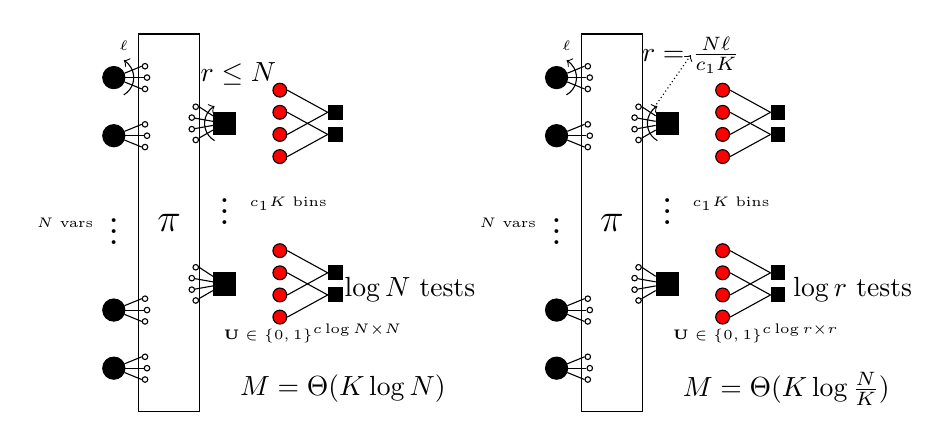
\begin{tikzpicture}
\def\emphsize{\normalsize}
\def\horzgap{40pt}; %Horizontal gap between nodes/levels
\def \gapVN{21pt}; %vertical gap between nodes
\def \gapCN{	29pt}; %Horizontal gap between nodes

\def \textoffs{9pt}; %Offset for writing r\leq N above cn4
\def\nodewidth{8pt};
\def\nodewidthsm{5pt}
\def\edgewidth{2pt};
\def\ext{12pt};
\def\moveX {20pt};
\def\moveYa{4pt}
\def\moveYb{12pt}
\def\arcradius{0.6*\ext}

\def\xmovement{4*\horzgap}

\def \n {8};
\def\ldeg{3};
\def \m {4};
\def\rdeg{6};
\def\langle{40};%120 degrees/3
\def\langle{20};%120 degrees/6

\tikzstyle{check} = [rectangle, draw,  inner sep=0mm, fill=black,minimum height=\nodewidth,minimum width=\nodewidth]
\tikzstyle{checksm} = [rectangle, draw, inner sep=0mm, fill=black,minimum height=\nodewidthsm, minimum width=\nodewidthsm]

\tikzstyle{bit} = [circle, draw, inner sep=0mm, fill=black, minimum size=\nodewidth]
\tikzstyle{bitsm} = [circle, draw, inner sep=0mm,fill=red, minimum size=\nodewidthsm]
\tikzstyle{edgesock} = [circle, inner sep=0mm, minimum size=\edgewidth,draw, fill=white]     

                          
\foreach \vn in {2,3,6,7}{
 \node[bit] (vn\vn) at (0,\vn*\gapVN) {};
\path (vn\vn) ++(20:\ext)node (evA\vn) [edgesock] {};
\path (vn\vn) ++(0:\ext) node (evB\vn) [edgesock] {};
\path (vn\vn) ++(-20:\ext) node (evC\vn) [edgesock] {};

  \draw (vn\vn) -- (evA\vn.west); 
  \draw (vn\vn) -- (evB\vn.west); 
  \draw (vn\vn) -- (evC\vn.west); 
}
\draw[->,thin] (vn7)++(-60:\arcradius) arc (-60:60:\arcradius)node[above]{\tiny{$\ell$}};

\path (vn3)--node(vndots) {\Large{$\vdots$}} (vn6);
\node[left =-0.2*\nodewidth of vndots](){\tiny{$N$ vars}};

\foreach \cn in {2,4}{
\node[check] (cn\cn) at (\horzgap,0.2in+\cn*\gapCN) {};

\path (cn\cn) ++(150:\ext) node (ecA\cn) [edgesock] {};
\path (cn\cn) ++(170:\ext) node (ecB\cn) [edgesock] {};
\path (cn\cn) ++(190:\ext) node (ecC\cn) [edgesock] {};
\path (cn\cn) ++(210:\ext) node (ecD\cn) [edgesock] {};

  \draw (cn\cn) -- (ecA\cn.east); 
  \draw (cn\cn) -- (ecB\cn);  
  \draw (cn\cn) -- (ecC\cn); 
    \draw (cn\cn) -- (ecD\cn); 
}

\draw[->,thin] (cn4)++(240:\arcradius) arc (240:120:\arcradius);
\path(cn4)++(5pt,2*\textoffs)node(){\emphsize{$r\leq N$}};
\path (cn2)--node(cndots) {\Large{$\vdots$}} (cn4);
\node [right=0.01*\nodewidth of cndots]{\tiny{$c_1K$ bins}};

\node[draw,minimum width=\horzgap-1.5*\ext,minimum height=6.5*\gapVN](perm) at (0.5*\horzgap,4.5*\gapVN){\Large{$\pi$}};

\foreach \cn in {2,4}{
\path (cn\cn) ++(\moveX,\moveYb) node (bitnA\cn) [bitsm] {};
\path (cn\cn) ++(\moveX,\moveYa) node (bitnB\cn) [bitsm] {};
\path (cn\cn) ++(\moveX,-\moveYa) node (bitnC\cn) [bitsm] {};
\path (cn\cn) ++(\moveX,-\moveYb) node (bitnD\cn) [bitsm] {};

\path (bitnB\cn) ++(\moveX,0) node (checknB\cn) [checksm] {};
\path (bitnC\cn) ++(\moveX,0) node (checknC\cn) [checksm] {};

\draw (bitnA\cn.east)--(checknB\cn.west);
\draw (bitnC\cn.east)--(checknB\cn.west);
\draw (bitnB\cn.east)--(checknC\cn.west);
\draw (bitnD\cn.east)--(checknC\cn.west);
}
\path(bitnD2)++(0.6*\moveX,-0.3*\moveX) node(){\tiny{$\mathbf{U}\in\{0,1\}^{c\log N \times N }$}};

\path (checknC2)++(3*\textoffs,0.5*\moveYa)node{\emphsize{$\log N$ tests}};
\node [below left=3*\nodewidth and 2*\nodewidth of bitnD2,anchor=west]{\emphsize{$M=\Theta(K\log N)$} };







\foreach \vn in {2,3,6,7}{
 \node[bit] (Bvn\vn) at (\xmovement,\vn*\gapVN) {};
\path (Bvn\vn) ++(20:\ext)node (BevA\vn) [edgesock] {};
\path (Bvn\vn) ++(0:\ext) node (BevB\vn) [edgesock] {};
\path (Bvn\vn) ++(-20:\ext) node (BevC\vn) [edgesock] {};

  \draw (Bvn\vn) -- (BevA\vn.west); 
  \draw (Bvn\vn) -- (BevB\vn.west); 
  \draw (Bvn\vn) -- (BevC\vn.west); 
}
\draw[->,thin] (Bvn7)++(-60:\arcradius) arc (-60:60:\arcradius)node[above]{\tiny{$\ell$}};

\path (Bvn3)--node(Bvndots) {\Large{$\vdots$}} (Bvn6);
\node[left =-0.2*\nodewidth of Bvndots](){\tiny{$N$ vars}};

\foreach \cn in {2,4}{
\node[check] (Bcn\cn) at (\xmovement+\horzgap,0.2in+\cn*\gapCN) {};

\path (Bcn\cn) ++(150:\ext) node (BecA\cn) [edgesock] {};
\path (Bcn\cn) ++(170:\ext) node (BecB\cn) [edgesock] {};
\path (Bcn\cn) ++(190:\ext) node (BecC\cn) [edgesock] {};
\path (Bcn\cn) ++(210:\ext) node (BecD\cn) [edgesock] {};

  \draw (Bcn\cn) -- (BecA\cn.east); 
  \draw (Bcn\cn) -- (BecB\cn);  
  \draw (Bcn\cn) -- (BecC\cn); 
  \draw (Bcn\cn) -- (BecD\cn); 
}

\draw[->,thin] (Bcn4)++(240:\arcradius) arc (240:120:\arcradius);
\draw[->,densely dotted](Bcn4)++(140:\arcradius)--++(14pt,20pt)node[](){\emphsize{$r=\frac{N\ell}{c_1K}$}};
\path (Bcn2)--node(Bcndots) {\Large{$\vdots$}} (Bcn4);
\node [right=0.01*\nodewidth of Bcndots]{\tiny{$c_1K$ bins}};

\node[draw,minimum width=\horzgap-1.5*\ext,minimum height=6.5*\gapVN](Bperm) at (\xmovement+0.5*\horzgap,4.5*\gapVN){\Large{$\pi$}};

\foreach \cn in {2,4}{
\path (Bcn\cn) ++(\moveX,\moveYb) node (BbitnA\cn) [bitsm] {};
\path (Bcn\cn) ++(\moveX,\moveYa) node (BbitnB\cn) [bitsm] {};
\path (Bcn\cn) ++(\moveX,-\moveYa) node (BbitnC\cn) [bitsm] {};
\path (Bcn\cn) ++(\moveX,-\moveYb) node (BbitnD\cn) [bitsm] {};

\path (BbitnB\cn) ++(\moveX,0) node (BchecknB\cn) [checksm] {};
\path (BbitnC\cn) ++(\moveX,0) node (BchecknC\cn) [checksm] {};

\draw (BbitnA\cn.east)--(BchecknB\cn.west);
\draw (BbitnC\cn.east)--(BchecknB\cn.west);
\draw (BbitnB\cn.east)--(BchecknC\cn.west);
\draw (BbitnD\cn.east)--(BchecknC\cn.west);
}
\path(BbitnD2)++(0.6*\moveX,-0.3*\moveX) node(){\tiny{$\mathbf{U}\in\{0,1\}^{c\log r\times r}$}};

\path (BchecknC2)++(3*\textoffs,0.5*\moveYa)node{\emphsize{$\log r$ tests}};
\node [below left=3*\nodewidth and 2*\nodewidth of BbitnD2,anchor=west]{\emphsize{$M=\Theta(K \log \frac{N}{K})$} };

\end{tikzpicture}}
\caption{Illustration of the main differences between SAFFRON \cite{lee2015saffron} on the left and our regular-SAFFRON scheme on the right. In both the schemes the peeling decoder on sparse graph requires $\Omega(K)$ bins. But for the bin decoder part, in SAFFRON scheme the right degree is a random variable with a maximum value of $N$ and thus requires $\Omega(\log N)$ tests at each bin. Whereas our scheme based on right-regular sparse graph has a constant right degree of $\Omega(\frac{N}{K})$ and thus requires only $\Omega(\log \frac{N}{K})$ tests at each bin. Thus we can improve the number of tests from $\Omega (K\log N)$ to order optimal $\Omega(K\log \frac{N}{K})$.}
\end{figure*}

\begin{definition}[Regular SAFFRON]
\label{Def:RegSaffron}
We define the ensemble of testing matrices for our scheme to be $\mc{G}_{l,r}(N,M_1)\times \mbf{U}_{r,p}$ where a graph $G$ is chosen from $\mc{G}_{l,r}(N,M_1)$, a signature matrix $\mbf{U}$ is chosen from $\mbf{U}_{r,p}$ and the testing matrix is defined as given in Eq. \eqref{Eqn:TestingMatrixDefn}. Note that the total number of tests for this testing scheme is $(2p+2)M_1\log r$ where $r=\frac{Nl}{M_1}$.
\end{definition}

For the regular SAFFRON testing ensemble defined in Def. \ref{Def:RegSaffron}, we employ the same peeling based decoder described in Sec.~\ref{Sec:PriorWork}. 

Now we consider the performance analysis of the regular SAFFRON scheme under the peeling based decoder. Similar to the SAFFRON scheme we will analyze the peeling decoder and the bin decoder separately and use union bound to bound the total error probability. As we have already  mentioned the analysis of just the peeling decoder can be carried out by considering a simplified peeling decoder on a pruned graph with only the non-zero variable nodes remaining. 

\begin{definition}[Pruned graph ensemble]
We will define the pruned graph ensemble $\tilde{\mc{G}}_{l,r}(N,K,M_1)$ as the set of all graphs obtained from removing a random $N-K$ subset of variable nodes from a graph from the ensemble $\mc{G}_{l,r}(N,M_1)$.
\end{definition}

Note that graphs from the pruned ensemble have $K$ variable nodes with a degree $l$ whereas the right degree is not regular anymore. 

\begin{lemma}[Edge d.d of pruned graph]
\label{Lem:EdgeDDPrunedGraph}
For the pruned graph ensemble $\tilde{\mc{G}}_{l,r}(N,K,M_1)$ it can be shown in the limit $K,N\rightarrow\infty$ that edge d.d coefficients $\rho_{1}=e^{-\lambda}$ and $\rho_{2}=\lambda e^{-\lambda}$ where $\lambda=l/c_1$ for the choice of $M_1=c_1K$, $c_1$ being some constant.
\end{lemma}

Note that even if our initial ensemble is left-and-right-regular the pruned graph has asymptotically same degree distribution as in the SAFFRON scheme where the initial graph is from left-regular ensemble.

\begin{lemma}
\label{Lem:PeelingRegularAnalysis}
For the pruned graph ensemble $\tilde{\mc{G}}_{l,r}(N, K,M_1)$ the oracle-based peeling decoder fails to peel off atleast $(1-\epsilon)$ fraction of the variable nodes with exponentially decaying probability for $M_1=c_1(\epsilon)K$ where $c_1(\epsilon)$ for various $\epsilon$ is given in Table. \ref{Table:constantsDE}.
\end{lemma}


\begin{proof}
From Lemma. \ref{Lem:EdgeDDPrunedGraph} we know that the edge degree distribution coefficients $\rho_1$ and $\rho_2$ are identical to that of the SAFFRON scheme and hence the same DE equations can be used here. Therefore the exact same proof as the proof of Lemma. \ref{Lem:PeelingAnalysisLeftRegular} can be employed here.
\end{proof}

\begin{theorem}
Let $p\in\Z$ such that $K$ and $N$ scale as $K\in o(N^{\frac{p}{p+1}})$. For $M=(2p+2)c_1(\epsilon)K \log_{2}\frac{N}{K}$, the regular SAFFRON framework we proposed, asymptotically, recovers atleast a $(1-\epsilon)$ fraction of the defective items for arbitrarily-small $\epsilon$ with high probability $1-O\left(\frac{K^{p+1}}{N^p}\right)$. Note that computational complexity of the decoding scheme is $O(K\log \frac{N}{K})$. The constant $c_1(\epsilon)$ is given in Table. \ref{Table:constantsDE}.
\end{theorem}
\begin{proof}
It remains to be shown that the total probability of error decays asymptotically in $K$ and $N$. Let $E_1$ be the event of oracle-based peeling decoder terminating without recovering atleast $(1-\epsilon)K$ variable nodes. Let $E_2$ be the event of the bin decoder making an error during the entirety of the peeling process and $E_{\tx{bin}}$ be the event of one instance of bin decoder making an error. The total probability of error $\tx{Pr}_e$ can be upper bounded by 
\begin{align*}
\tx{Pr}_e &\leq \tx{Pr}(E_1)+ \tx{Pr}(E_2)\\
               &\leq \tx{Pr}(E_1)+ Kl\tx{Pr}(E_{\tx{bin}})\\
               &\in O\left(\frac{K^{p+1}}{N^p}\right)
\end{align*}
where the second inequality is due to the union bound over a maximum of $Kl$ instances of bin decoding. The third line is due to the fact that $\tx{Pr}(E_1)$ is exponentially decaying in $K$ (see Lemma. \ref{Lem:PeelingRegularAnalysis}) and $\tx{Pr}(E_{\tx{bin}})=(\frac{c_1K}{Nl})^p$ (see Lemma. \ref{Lem:BinDecoderAnalysis} and Def. \ref{Def:RegSaffron})
\end{proof}

\begin{proof}[Proof of Lem. \ref{Lem:EdgeDDPrunedGraph}]
We will first derive $R(x)$ for the pruned graph ensemble and then use the relation\cite{richardson2008modern} $\rho(x)=\frac{R'(x)}{R'(1)}$ to derive the edge d.d . Note that all the check nodes have a uniform degree $r$ before pruning. When pruning we are removing a $N-K$ subset of variable nodes at random i.e., asymptotically this is equivalent to removing each edge from the graph with a probability $1-\epsilon$ where $\epsilon\coleq \frac{K}{N}$. Under this process the right-node d.d can be written as
\begin{align*}
R_1&=r\epsilon(1-\epsilon)^{r-1},\quad \text{ and similarly}\\
R_i &=\binom{r}{i} \epsilon^{i}(1-\epsilon)^{r-i},
\end{align*}
thus giving us $R(x)=(\epsilon x+(1-\epsilon))^{r}$. This gives us 
\begin{align*}
\rho(x)&=\frac{r\epsilon(\epsilon x+(1-\epsilon))^{r-1}}{r\epsilon}\\
          &=(\epsilon x+(1-\epsilon))^{r-1}.
\end{align*}
Thus we can compute that $\rho_1=(1-\epsilon)^{r-1}$ and $\rho_2=(r-1)\epsilon(1-\epsilon)^{r-2}$. We evaluate these quantities asymptotically as $K,N\rightarrow \infty$ and $M_1=CK$.
\begin{align*}
\lim_{K,N\rightarrow \infty} \rho_1&=\lim_{K,N\rightarrow \infty} (1-\frac{K}{N})^{\frac{Nl}{CK}-1}\\
&=e^{-\lambda} \qquad \text{ where } \lambda=\frac{l}{C}
\end{align*}
Similarly we can show $\lim_{K,N\rightarrow \infty}\rho_2=\lambda e^{-\lambda}$.
\end{proof}

\begin{figure}
\label{Fig:SimulationNoiseless}
\begin{center}
\resizebox{\columnwidth}{!}{% This file was created by matlab2tikz v0.4.7 running on MATLAB 7.14.
% Copyright (c) 2008--2014, Nico Schlömer <nico.schloemer@gmail.com>
% All rights reserved.
% Minimal pgfplots version: 1.3
% 
% The latest updates can be retrieved from
%   http://www.mathworks.com/matlabcentral/fileexchange/22022-matlab2tikz
% where you can also make suggestions and rate matlab2tikz.
% 
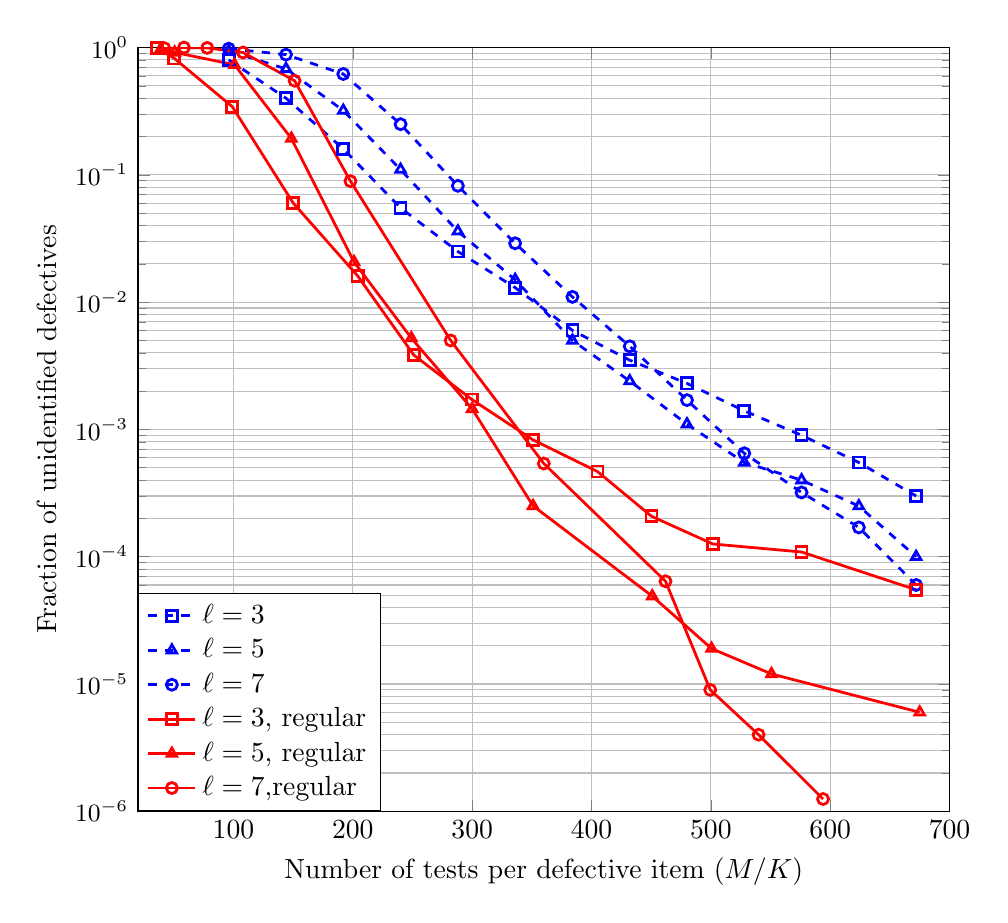
\begin{tikzpicture}
\def\fsize{\normalsize}
\pgfplotsset{every y tick label/.append style={font=\footnotesize}}
\pgfplotsset{every y tick label/.append style={font=\small}}

\begin{axis}[%
width=0.85\columnwidth,
height=0.8\columnwidth,
scale only axis,
xmin=20,
xmax=700,
xtick = {100,200,...,700},
xmajorgrids,
ymode=log,
ymin=1e-06,
ymax=1,
yminorticks=true,
ymajorgrids,
yminorgrids,
xlabel={\fsize{Number of tests per defective item ($M/K$)}},
ylabel={\fsize{Fraction of unidentified defectives}},
legend style={at={(0,0)},anchor=south west,draw=black,fill=white,legend cell align=left,font=\fsize}
]
\addplot [color=blue,dashed, mark=square,mark options={solid},line width=1pt]
  table[row sep=crcr]{96	0.8\\
144	0.4\\
192	0.16\\
240	0.055\\
288	0.025\\
336	0.013\\
384	0.006\\
432	0.0035\\
480	0.0023\\
528	0.0014\\
576	0.0009\\
624	0.00055\\
672	0.0003\\
};
\addlegendentry{$\ell=3$};

\addplot [color=blue,dashed,line width=1pt,mark=triangle,mark options={solid}]
  table[row sep=crcr]{96	0.94\\
144	0.68\\
192	0.32\\
240	0.11\\
288	0.036\\
336	0.015\\
384	0.005\\
432	0.0024\\
480	0.0011\\
528	0.00055\\
576	0.0004\\
624	0.00025\\
672	0.0001\\
};
\addlegendentry{$\ell=5$};


\addplot [color=blue,dashed,mark=o,mark options={solid},line width=1pt]
  table[row sep=crcr]{96	0.98\\
144	0.88\\
192	0.62\\
240	0.25\\
288	0.082\\
336	0.029\\
384	0.011\\
432	0.0045\\
480	0.0017\\
528	0.00065\\
576	0.00032\\
624	0.00017\\
672	6e-05\\
};
\addlegendentry{$\ell=7$};

%\addplot [color=blue,dashed,line width=3pt,mark=square,mark options={solid}]
%  table[row sep=crcr]{96	0.98\\
%144	0.94\\
%192	0.85\\
%240	0.52\\
%288	0.21\\
%336	0.065\\
%384	0.024\\
%432	0.0095\\
%480	0.0032\\
%528	0.0014\\
%576	0.00055\\
%624	0.00024\\
%672	0.0002\\
%};
%\addlegendentry{$l=9$};

\addplot [color=red,solid, line width=1pt, mark=square,mark options={solid}]
  table[row sep=crcr]{
36  0.99261\\
50.40      8.22e-1 \\
99.00      3.43e-1\\
150.00    6.01e-2 \\
204.00    1.61e-2\\
251.10    3.84e-3 \\
299.70    1.72e-3  \\
 351.00    8.28e-4 \\ 
 405.00    4.67e-4\\
 450.24    2.08e-4\\
 501.60  1.26e-4 \\  
 576.00  1.09e-4\\
672.00   5.50e-5\\
%66  0.80679\\
%79.20  0.65094\\
%99  0.4133 \\
%120     0.1596\\
%150     0.06312\\
%180 0.02797\\ 
%210     0.01396\\
%253.8  0.00344 \\
%307.8  0.00153\\
%324     0.00124 \\
%361.8  0.00078 \\
%369.6  0.00046 \\
%408     0.00031\\
%480.0  0.00021 \\
%672 0.000076\\
};
\addlegendentry{$\ell=3$, regular};

\addplot [color=red, solid, line width=1pt, mark=triangle,mark options={solid}]
  table[row sep=crcr]{
   39.000    0.970769\\
    50.700      9.16e-1   \\
100.800     7.33e-1   \\
148.500     1.93e-1   \\
201.000     2.07e-2  \\
249.000     5.22e-3  \\
300.000     1.450e-3\\
351.000     2.51e-4\\
%405.000     8.60e-5\\
450.900     4.90e-5\\
500.580     1.90e-5 \\
550.800     1.20e-5\\
%602.100 	  1.10e-5\\
675.000     6.00e-6\\
%   72.000    0.946226\\
% 132.000    0.327190\\
% 198.000    0.036304 \\
% 210.000    0.015015 \\
% 240.000    0.006573\\
% 270.000    0.003021\\
% 300.000    0.001460\\
% 360.000    0.000479\\
% 378.000    0.000157\\
% 453.600    0.000048\\
% 540.000    0.000013\\
% 604.800    0.000003\\
 };
\addlegendentry{$\ell=5$, regular};

\addplot [color=red, solid, line width=1.0pt,mark=o]
  table[row sep=crcr]{
42.00  0.99      \\
58.50	0.9995  \\
78.00    0.9937 \\
108.00   0.9142 \\
151.20  0.5487  \\
198.00 8.92e-2  \\
282.00  5.0e-3    \\
360.00  5.4e-4   \\
462.00  6.42e-5   \\
499.50  9.00e-6   \\
540.00  4.00e-6   \\
594.00  1.25e-6   \\
};
\addlegendentry{$\ell=7$,regular};

\end{axis}
\end{tikzpicture}%}
\caption{MonteCarlo simulations for $K=100, N=2^{16}$. We compare the SAFFRON scheme with our regular SAFFRON scheme for various left degrees $l\in\{3,5,7\}$. For a given $l$ the bin detection size is fixed and we vary the number of bins. The plots in blue indicate the SAFFRON scheme and the plots in red indicate our regular SAFFRON scheme based on left-and-right-regular bipartite graphs.}
\end{center}
\end{figure}

\section{Robust Group Testing}
In this section we extend our scheme to the group testing problem where the test results can be noisy. To be formal, the signal model looks like
\begin{align*}
\mbf{y=A}\odot \mbf{x+w},
\end{align*}
where the addition is over binary field and $\mbf{w}\in\{0,1\}^N$ is an i.i.d noise vector distributed according to Bernoulli distribution with parameter $0<q<\frac{1}{2}$.

\subsection*{Testing Scheme}
In \cite{lee2015saffron} for the robust group testing problem, the signature matrix used for noiseless group testing problem is modified using a error control coding such that it can handle singletons and resolvable doubletons in the presence of noise. The binning operation as definied by the bipartite graph is exactly identical to that of noiseless case. We state the modification to the signature matrix and new bin detection decoding scheme as given in \cite{lee2015saffron} for the sake of completeness and then state the performance bounds for our scheme for the noisy group testing problem.

Let $\mc{C}_n$ be a binary error-correcting code with the following definition:
\begin{itemize}
\item Let the encoder and decoder functions be $f:\{0,1\}^{n}\rightarrow \{0,1\}^{\frac{n}{R}}$ and $g:\{0,1\}^{\frac{n}{R}}\rightarrow \{0,1\}^{n}$ respectively where $R$ is the rate of the code.
\end{itemize}
We can use any error-correcting code but for ease of analysis and tight upper bound for the number of tests we will use spatially-coupled LDPC codes which are known to be capacity achieving \cite{kumar2014threshold,kudekar2013spatially}.For spatially-coupled LDPC codes, being capacity achieving is equivalent to: 
\begin{itemize}
\item There exists a sequence of codes $\{\mc{C}_n\}$ with the rate of each code being $R$ satisfying 
\begin{align}
\label{Eqn:ProbErrorCoding}
R<1-H(q)-\delta=1+q\log_2 q+(1-q)\log_2(1-q)-\delta
\end{align}
%where $H(q)=-q\log_2 q-(1-q)\log_2(1-q)$, 
for any arbitrary small constant $\delta$ such that the probability of error $\text{Pr}\left(g(\mbf{x+w})\neq \mbf{x}\right)<2^{\kappa n}$ for some $\kappa >0$.
\end{itemize} 
The modified signature matrix $\mbf{U}'_{r,p}$ can be described via $\mbf{U}_{r, p}$ given in Eq. \eqref{Eqn:SignatureMatrix}, and encoding function $f$ for a code $\mc{C}_{\log_2 r}$ as follows:
 \begin{align}
\label{Eqn:SignatureMatrixModified}
\mbf{U}_{r,p}'\coleq\begin{bmatrix}
f(\mbf{b}_1)  & f(\mbf{b}_2) &\cdots & f(\mbf{b}_r) \\
\overline{f(\mbf{b}_1)} & \overline{f(\mbf{b}_2)} & \cdots & \overline{f(\mbf{b}_r)}\\
f(\mbf{b}_{\pi^{1}_{1}}) & f(\mbf{b}_{\pi^{1}_{2}}) & \cdots & f(\mbf{b}_{\pi^{1}_{r}})\\
\overline{f(\mbf{b}_{\pi^{1}_{1}})} & \overline{f(\mbf{b}_{\pi^{1}_{2}})} & \cdots & \overline{f(\mbf{b}_{\pi^{1}_{r}})}\\
\cdots &  &\vdots \\
f(\mbf{b}_{\pi^{p}_{1}}) & f(\mbf{b}_{\pi^{p}_{2}}) & \cdots & f(\mbf{b}_{\pi^{p}_{r}})\\
\overline{f(\mbf{b}_{\pi^{p}_{1}})} & \overline{f(\mbf{b}_{\pi^{p}_{2}})} & \cdots & \overline{f(\mbf{b}_{\pi^{p}_{r}})}\\
\end{bmatrix}
\end{align}  
Then the overall testing matrix $\mbf{A}$ is defined in identical fashion to the definition in Sec. \ref{Sec:PriorWork} for the case of noiseless case except that $\mbf{U}$ will be replaced by $\mbf{U'}$. Formally it can be defined as $\mbf{A}\coleq [\mbf{A}_{1}^{T},\ldots,\mbf{A}_{M_{1}}^{T}]^T$ where $\mbf{A}_{i}=\mbf{U'} \diag (\mbf{t}_i)$ where the binary vectors $\mbf{t}_i$ are defined in Sec. \ref{Sec:PriorWork}. 

\subsection*{Decoding}
Describe error-control coding in one para using function $g$.


\subsection*{Results}
\begin{lemma}[Robust Bin Decoder Analysis]
For a signature matrix $\mbf{U'}_{r,p}$ as described in \eqref{Eqn:SignatureMatrixModified}, the robust bin decoder misses a singleton with probability no greater than $\frac{3}{r^{\kappa}}$. The robust bin decoder wrongly declares a singleton with probability no greater than $\frac{1}{r^{p\kappa}}$.
\end{lemma}
The fraction of missed singeltons will be compensated by using $M(1+\frac{3}{r^{\kappa}})$ instead of $M$ such that the total number of singletons decoded will be $M(1+\frac{3}{r^{\kappa}})(1-\frac{3}{r^{\kappa}})\approx M$.

\begin{theorem}
Let $p\in\Z$ such that $K$ and $N$ scale as $K\in o\left(N^{\frac{p\kappa}{p\kappa+1}}\right)$ where $\kappa>0$ is defined in Eq. \eqref{Eqn:ProbErrorCoding}. For $M=2(p+1)\beta(q)c_1(\epsilon)K \log_{2}\frac{N}{K}$, the robust regular SAFFRON framework we proposed, asymptotically, recovers atleast a $(1-\epsilon)$ fraction of the defective items for arbitrarily-small $\epsilon$ with high probability $1-O\left(\frac{K^{p\kappa+1}}{N^{p\kappa}}\right)$. Here $\beta(q)=\frac{1}{R}>\frac{1}{1-H(q)-\delta}$ for an arbitrary small constant $\delta$ and the constants $c_1(\epsilon)$ are given in Table. \ref{Table:constantsDE}. Note that computational complexity of the decoding scheme is $O(K\log \frac{N}{K})$.
\end{theorem}

\bibliographystyle{ieeetr}
\bibliography{journal_full,sparseestimation}
\end{document} 